% !TeX document-id = {63e2cb4c-39e5-4fe5-ae31-d450d2286238}
% !TeX TXS-program:compile = txs:///pdflatex/[--shell-escape]
\documentclass[11pt,a4paper]{exam}
\printanswers % pour imprimer les réponses (corrigé)
%\noprintanswers % Pour ne pas imprimer les réponses (énoncé)
\addpoints % Pour compter les points
\usepackage[utf8]{inputenc}
\usepackage{minted}

\usepackage{algorithm} % pour faire du pseudo-code
\usepackage{algorithmicx} % pour faire du pseudo-code
\usepackage{algpseudocode} % pour faire du pseudo-code

% Traduction des commandes en pseudo-code
\renewcommand{\algorithmicfor}{\textbf{pour}}
\renewcommand{\algorithmicif}{\textbf{si}}
\renewcommand{\algorithmicthen}{\textbf{alors}}
\renewcommand{\algorithmicelse}{\textbf{sinon}}
\renewcommand{\algorithmicfunction}{\textbf{fonction}}
\renewcommand{\algorithmicforall}{\textbf{pour tout}}
\renewcommand{\algorithmicdo}{\textbf{faire}}
\renewcommand{\algorithmicwhile}{\textbf{tant que}}
\renewcommand{\algorithmicend}{\textbf{fin}}
\renewcommand{\algorithmicreturn}{\textbf{retourner}}
\renewcommand{\algorithmicrequire}{\textbf{Entrée:}}
\renewcommand{\algorithmicensure}{\textbf{Sortie:}} % Détournement du Ensure, mais ce n'est pas très grave...

\usepackage{geometry}
\usepackage{amsmath,amssymb}
\usepackage{multicol}
\usepackage{graphicx}
\usepackage{setspace}
\usepackage{dashundergaps}
%\usepackage[monochrome]{xcolor} % Permet de tout mettre en N&B strict
\usepackage{xcolor}
%\selectcolormodel{gray} % Permet de tout mettre en niveaux de gris
\geometry{left=0.7cm, right=0.7cm, top=1.5cm, bottom=1cm} % Définition des marges du doc

%\newcommand{\class}{1\textsuperscript{ère} Spé. NSI Gr. 2\textsubscript{A}}
\newcommand{\class}{1\textsuperscript{ère} Spé. NSI Gr. 2}
\newcommand{\examnum}{Contrôle \#4}
\newcommand{\examdate}{05/04/2024}
\newcommand{\timelimit}{1 Heure}
\newcommand{\lycee}{Lycée Fustel de Coulanges}

\pagestyle{head}
\firstpageheader{}{}{}
\runningheader{\class}{\examnum\ - Page \thepage\ / \numpages}{\examdate}
\runningheadrule


\begin{document}
% Espace d'en-tête
    \noindent
    \begin{spacing}{1}
        \noindent
        \begin{tabular*}{\textwidth}{l @{\extracolsep{\fill}} l @{\extracolsep{6pt}} l}
            \textbf{\class} & \textbf{\examnum, \examdate}&\\
            \textbf{\lycee} &\textbf{Durée: \timelimit} &\\
        \end{tabular*}\\
    \end{spacing}

    \noindent
    \vspace{10pt}
    \hrule
    \vspace{5pt} 
    \noindent
    \\
    Ce contrôle comporte \numquestions\ questions; le nombre maximal possible de points est de \numpoints. 
    Les réponses sont à porter sur une copie \uline{comportant votre nom}.
    Il n'est pas nécessaire de répondre aux questions dans l'ordre \textemdash\ commencez par celles où vous vous sentez le plus à l'aise \textit{(mais ne tentez les questions bonus qu'après avoir fini le reste!!)}.\\
    Les calculatrices ne sont \uline{pas} autorisées.\\
    \noindent
    \hrule
    \vspace{15pt} 

    \begin{questions} % DEBUT DE L'EXAMEN
		\begin{spacing}{1}
    
		\question \textit{Questions de cours}
		\begin{parts}
			\part[1 \half]{QCM -- les réponses sont à porter sur votre copie; il n'est pas nécessaire de justifier vos réponses; il y a une bonne réponse par question}
			\begin{subparts}
			
				\subpart Si j'ai déterminé qu'un algorithme était de complexité quadratique (également noté $\mathcal{O}(n^2)$), et si je double la taille des données en entrée, alors la durée de traitement...
				\begin{checkboxes}
					\choice ... restera la même.
					\choice ... doublera.
					\choice ... triplera.
					\correctchoice ... quadruplera.
				\end{checkboxes}
				\begin{minted}
					[
					bgcolor = gray!15,
					fontsize = \footnotesize,
					linenos = true % numéros de ligne
					]
					{Python}
def compte_elts(liste):
    compteur = 0
    for element in liste:
        compteur += 1
    return compteur
				\end{minted}
				\subpart La fonction ci-dessus a une complexité en ($n$ étant la taille de \texttt{liste})...
				\begin{checkboxes}
					\choice ... $\mathcal{O}(n^2)$.
					\correctchoice ... $\mathcal{O}(n)$.
					\choice ... $\mathcal{O}(log_2(n))$.
					\choice ... $\mathcal{O}(1)$
				\end{checkboxes}
				\subpart Un tri "stable"...
				\begin{checkboxes}
					\correctchoice ... maintient les positions relatives des éléments équivalents.
					\choice ... place les éléments en ordre décroissant.
					\choice ... a une complexité supérieure à un tri instable.
					\choice  ... a une complexité inférieure à un tri instable.
				\end{checkboxes}
				\end{subparts}
			
			\part[2] Expliquez en deux ou trois phrases le principe d'une approche gloutonne à la résolution d'un problème.
			\begin{solution}
				Les éléments de réponse attendus étaient (tous n'étaient pas obligatoirement à intégrer à votre réponse):
				\begin{itemize}
					\item Une approche gloutonne vise à résoudre des problèmes d'optimisation -- c'est-à-dire qu'ils ne recherchent pas \textit{la} solution à un problème, mais la solution \textit{la meilleure possible} (selon un axe d'optimisation défini) à ce problème.
					\item Une approche gloutonne est une méthode de résolution qui fait, à chaque étape, le choix le plus avantageux à court terme ou le plus "gourmand" sans prendre en compte les conséquences futures. Ce choix est fait dans l'espoir qu'il mènera à une solution globale optimale du problème.
					\item On parle d'\textit{optima locaux} -- ce qui décrit la notion de "meilleur choix" local, pour chaque étape prise individuellement.
					\item Les algorithmes gloutons ne fournissent pas nécessairement la meilleure solution possible -- mais ils peuvent le faire dans certains cas, comme celui du rendu de monnaie caractérisé par le fait que l'ensemble des solutions possibles (l'ensemble des dénominations possibles en euros) constitue un \textit{système canonique}.
				\end{itemize}
			\end{solution}

			\part[2] Supposons que la fonction \texttt{recherche\_dicho(table, elt)} implémente la recherche dichotomique telle que nous l'avons étudiée en cours. Quelles sont les valeurs qui vont être examinées lors de l'appel \texttt{recherche\_dicho([0, 1, 1, 2, 3, 5, 8, 9, 11], 7}? \textit{Indice: la première va être table[4] qui vaut 3.}\footnote{N'hésitez pas à utiliser sur votre copie un tableau donnant les valeurs successives des indices "\texttt{debut}", "\texttt{fin}", et "\texttt{milieu}".}
			
			\begin{solution}
				Comme suggéré par l'énoncé, utilisons la technique du tableau de valeurs que nous avons déjà utilisée en cours:
				\definecolor{mongreen}{RGB}{8,180,84}
				\begin{center}				
					\begin{figure}[H]
						\centering
						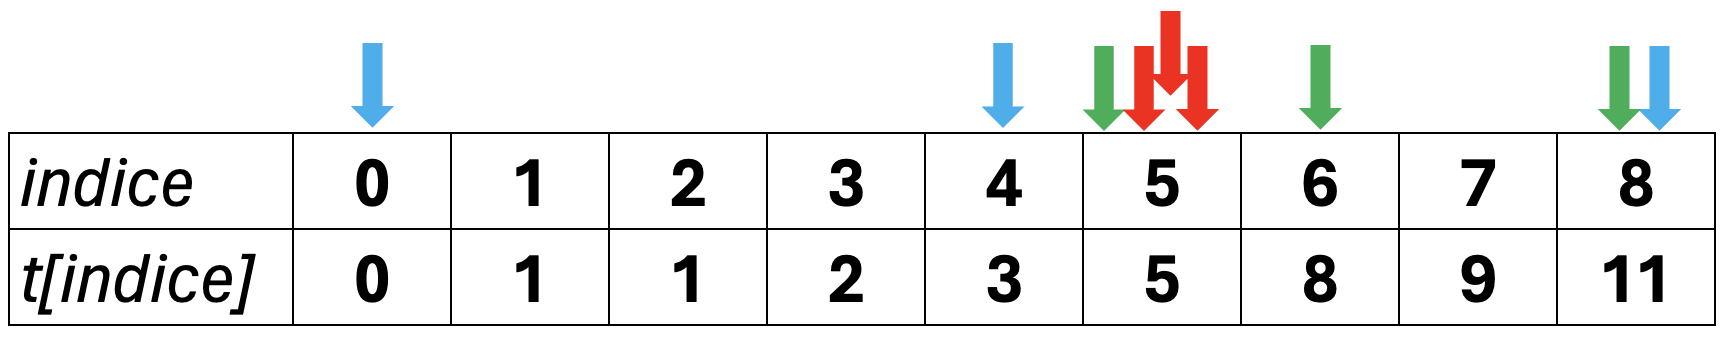
\includegraphics[width=0.6\textwidth]{RechDich.png}
					\end{figure}
					
					\begin{tabular}{|c|c|c|c|}
						\hline
						\textbf{Debut} & \textbf{Fin} & \textbf{Milieu} & \textbf{\texttt{table[Milieu]}}\\
						\hline
						\textbf{\textcolor{blue}{0}} & \textbf{\textcolor{blue}{8}} & \textbf{\textcolor{blue}{4}} & \textbf{\textcolor{blue}{3}}\\
						\hline 
						\textbf{\textcolor{mongreen}{5}} & \textbf{\textcolor{mongreen}{8}} & \textbf{\textcolor{mongreen}{6}} & \textbf{\textcolor{mongreen}{8}} \\
						\hline 
						\textbf{\textcolor{red}{5}} & \textbf{\textcolor{red}{5}} & \textbf{\textcolor{red}{5}} & \textbf{\textcolor{red}{5}} \\
						\hline
					\end{tabular}
				\end{center}
				
				\vspace{\baselineskip}
				Le tableau ci-dessus montre bien que trois valeurs sont examinées successivement par l'algorithme avant d'arriver à la conclusion de l'absence de l'élément 7 dans la table fournie en entrée. Ces trois valeurs sont (c'est évidemment toujours \texttt{t[milieu]} qui est évalué --- voir le cours sur l'algorithme de recherche dichotomique si cela ne vous parait pas clair):
				\begin{enumerate}
					\item \texttt{t[4] = 3}
					\item \texttt{t[6] = 8}
					\item \texttt{t[5] = 5}
				\end{enumerate}
			\end{solution}
		\end{parts}
			
		\question[6]{\textit{Détermination de complexités}}
		\newcommand{\lgcode}{0.31}
		
		\noindent
		\begin{tabular}{c c c}
			\begin{minipage}{\lgcode\linewidth}
				\begin{minted}[
					bgcolor=gray!15,
					fontsize=\footnotesize,
					linenos % Numéros de ligne
					]{python}
def f1(n):
    x = 0
    for i in range(n):
        x = x + 1
    return x
				\end{minted}
			\end{minipage}
			&
			\begin{minipage}{\lgcode\linewidth}
				\begin{minted}[
					bgcolor=gray!15,
					fontsize=\footnotesize,
					linenos % Numéros de ligne
					]{python}
def f2(n):
    x = 0
    for i in range(1000000000):
        x = x + 1
    return x
				\end{minted}
			\end{minipage}
			&
			\begin{minipage}{\lgcode\linewidth}
				\begin{minted}[
					bgcolor=gray!15,
					fontsize=\footnotesize,
					linenos % Numéros de ligne
					]{python}
def f3(n):
    x = 0
    for i in range(n):
        for j in range(5):
            x = x + 1
    return x
				\end{minted}
			\end{minipage}
			\\
			\begin{minipage}{\lgcode\linewidth}
				\begin{minted}[
					bgcolor=gray!15,
					fontsize=\footnotesize,
					linenos % Numéros de ligne
					]{python}
def f4(n):
    x = 0
    i = 0
    while i * i < n:
        x = x + 1
        i = i + 1
    return x
				\end{minted}
			\end{minipage}
			&
			\begin{minipage}{\lgcode\linewidth}
				\begin{minted}[
					bgcolor=gray!15,
					fontsize=\footnotesize,
					linenos % Numéros de ligne
					]{python}
def f5(n):
    x = 0
    for i in range(n):
        for j in range(n):
            x = x + 1
    return x
				\end{minted}
			\end{minipage}
			&
			\begin{minipage}{\lgcode\linewidth}
				\begin{minted}[
					bgcolor=gray!15,
					fontsize=\footnotesize,
					linenos % Numéros de ligne
					]{python}
def f6(n):
    x = 0
    for i in range(n):
        x = x + 1
    for j in range(n):
        x = x + 1
    return x
				\end{minted}
			\end{minipage}
		\end{tabular}
		
		Déterminer la complexité de chacune des fonctions \texttt{f1} à \texttt{f6} en fonction de $n$ (vous pouvez utiliser la notation $\mathcal{O}()$ ou la terminologie "constante / linéaire / quadratique / autre"). Il est demandé pour chaque fonction une brève phrase de justification de la réponse.
		
		\begin{solution}
			Les complexités respectives de ces fonctions sont:
			\begin{description}
				\item[f1] $i$ parcourt toutes les valeurs de $0$ à $(n-1)$, donc la complexité est \textbf{linéaire} en $\mathcal{O}(n)$; on se convainc aisément en effet que si $n$ double, alors le nombre d'itérations de la boucle doublera aussi.
				\item[f2] $n$ n'apparait même pas dans la fonction -- la complexité de celle-ci n'en dépend donc absolument pas, on est donc sur une complexité \textbf{constante}, en $\mathcal{O}(1)$; on se convainc aisément en effet que si $n$ double, alors le nombre d'itérations de la boucle ne changera pas --- il restera à 1.000.000.000.
				\item[f3] Il y avait ici un (tout petit) piège: on a bien deux boucles imbriquées, mais le nombre d'itérations de la boucle intérieure est fixe (à 5), donc ne dépend pas de $n$; la complexité dépend donc exclusivement de la boucle extérieure pour laquelle $i$ parcourt toutes les valeurs de $0$ à $(n-1)$, donc la complexité est \textbf{linéaire} en $\mathcal{O}(n)$; on se convainc aisément en effet que si $n$ double, alors le nombre d'itérations de la boucle doublera aussi.
				\item[f4] La fonction la plus difficile des 6: $i \times i$ évolue de $0$ à $(n-1)$, donc i lui même évolue, de 1 en 1, de $0$ à approximativement $\sqrt{n}$. Le nombre d'itérations de la boucles dépend donc de la racine carrée de $n$ -- et sa complexité est donc en $\mathcal{O}(\sqrt{n})$. On se convainc d'ailleurs aisément que si $n$ double, alors le nombre d'itérations de la boucle passera d'environ $\sqrt{n}$ à $\sqrt{2n}$ -- et aura donc été multiplié par $\sqrt{2}$.
				\item[f5] Là nous nous trouvons dans une configuration de boucles imbriquées "classique" où la boucle intérieure accomplit $n$ itérations pour chaque itération de la boucle extérieure qui en accomplit elle-même $n$ également -- on est donc dans une complexité \textbf{quadratique} en $\mathcal{O}(n^2)$; on se convainc aisément en effet que si $n$ double, alors le nombre d'itérations de la boucle intérieure doublera, celui de la boucle extérieure également et donc au total le nombre d'opérations aura quadruplé (aura donc été multiplié par $2^2$).
				\item[f6] Pas de piège en tant que tel ici mais quelque chose à retenir: la complexité est une question d'augmentation en fonction de la taille de l'entrée -- donc une fonction qui réalise $n$ opérations et une qui en réalise $2 \times n$ comme, à l'évidence, celle-ci, ont la même complexité puisqu'un doublement de $n$ reviendra à un doublement du nombre d'opérations: complexité \textbf{linéaire} en $\mathcal{O}(n)$.
			\end{description}
		\end{solution}

        \question[2]{\textit{Fonction de recherche de 0}}
        \begin{minted}
        	[
        	bgcolor = gray!15,
        	fontsize = \footnotesize,
        	linenos = true % numéros de ligne
        	]
        	{Python}
def compter_zeros(t):
''' Fonction qui compte le nombre de zéros après chaque élément de t'''
    n = len(t)
    compte = [0] * n # Rappel: renvoie un tableau de longueur n de 0: [0, 0, ..., 0]
    for i in range(n):
        for j in range(i+1, n):
            if t[j] == 0:
                compte[i] += 1
    return compte
    \end{minted}
       	Exécutons cette fonction sur un tableau spécifique: \texttt{compter\_zeros([1, 0, 2, 0])}. Sur votre copie, complétez le tableau suivant avec les valeurs successives des variables -- ajoutez autant de lignes qu'il y aura de passages dans la comparaison de la ligne 7 "\texttt{if t[j] == 0:}"\footnote{Indice: il y en aura 6 en tout, les deux déjà présents dans l'énoncé inclus.}; puis concluez en indiquant ce que renverra la fonction.
       	
       	\begin{tabular}{|c|c|c|c|c|c|}
       		\hline
       		\textbf{Ligne Code} & \texttt{compte} & \texttt{i} & \texttt{j} & \texttt{t[i]} & \texttt{t[j]} \\
       		\hline
       		7 & \texttt{[0,0,0,0]} & 0 & 1 & 1 & 0\\
       		\hline 
       		7 & \texttt{[1,0,0,0]} & 0 & 2 & 1 & 2\\
       		\hline 
       		7 & ... & ... & ... & ... & ...\\
       		\hline 
       	\end{tabular}
        \begin{solution}
        	
        	\begin{tabular}{|c|c|c|c|c|c|}
        		\hline
        		\textbf{Ligne Code} & \texttt{compte} & \texttt{i} & \texttt{j} & \texttt{t[i]} & \texttt{t[j]} \\
        		\hline
        		7 & \texttt{[0,0,0,0]} & 0 & 1 & 1 & 0\\
        		\hline 
        		7 & \texttt{[1,0,0,0]} & 0 & 2 & 1 & 2\\
        		\hline 
        		7 & \texttt{[1,0,0,0]} & 0 & 3 & 1 & 0\\
        		\hline 
        		7 & \texttt{[2,0,0,0]} & 1 & 2 & 0 & 2\\
        		\hline 
        		7 & \texttt{[2,0,0,0]} & 1 & 3 & 0 & 0\\
        		\hline 
        		7 & \texttt{[2,1,0,0]} & 2 & 3 & 2 & 0\\
        		\hline 
        	\end{tabular}
        	
        	Lors du dernier passage dans le test "\texttt{if t[j] == 0:}" la condition sera satisfaite (puisque \texttt{t[3] = 0}), donc la fonction renverra comme tableau final \texttt{[2, 1, 1, 0]}.
        \end{solution}
		
		\question{\textit{Fichier CSV}} --- On considère le code suivant:
		\begin{minted}
			[
				bgcolor = gray!15,
				fontsize = \footnotesize,
				linenos = true % numéros de ligne
			]
			{Python}
import csv
fichier = open('Specialites.csv', 'r', encoding = 'utf-8')
table = list(csv.DictReader(fichier))
		\end{minted}
		Et soit le fichier \texttt{Specialites.csv} contenant les données suivantes:
		\begin{verbatim}
			Eleve,Classe,Age,Spe1,Spe2,Spe3
			Loubna,1G5,16,Maths,NSI,Physique
			Olivier,1G2,17,NSI,Maths,SES
			Lenny,1G2,17,LLC-Anglais,SES,NSI
			Anju,1G3,16,LLC-Anglais,NSI,SES
			Sophie,1G5,15,Maths,NSI,SES
		\end{verbatim}
		\begin{parts}
			\part[\half] Qu'est-ce qui va s'afficher à l'exécution du code suivant?
			\begin{minted}
				[
					bgcolor = gray!15,
					fontsize = \footnotesize,
					linenos = true % numéros de ligne
				]
				{Python}
for i in range(len(table)):
    print(table[i]['Spe2'])
			\end{minted}
			\begin{solution}
				Pas de difficulté particulière ici -- juste un affichage des valeurs successives de la colonne \text{Spe2}, donc:
				
				\begin{verbatim}
					NSI
					Maths
					SES
					NSI
					NSI
				\end{verbatim}
			\end{solution}
			\part[1] Complétez la fonction suivante pour qu'elle fasse ce qui est spécifié.
			\begin{minted}
				[
				bgcolor = gray!15,
				fontsize = \footnotesize,
				linenos = true % numéros de ligne
				]
				{Python}
def CompteEleves(spe, table):
    ''' Fonction qui renvoie le nombre d'élèves ayant choisi la spécialité passée en argument'''
    n = len(table)
    compte = 0
    for i in range(n):
    	# A COMPLETER: le "if" qui va tester si l'élève d'indice i a la spécialité "spe"
    	...
    	    compte += 1
    return compte
			\end{minted}
			\part[2] Rédigez une fonction AgeMoy(classe) qui renvoie l'âge moyen des élèves présents dans la classe passée en argument. Par exemple \texttt{AgeMoy('1G5')} renverra la valeur $15.5$ (la moyenne de 15 et 16)\footnote{N'hésitez pas à commencer par en rédiger l'algorithme en pseudo-code: des points seront attribués à cela même si le code final est faux ou absent.}.
		\end{parts}
		
		\vspace{\baselineskip}
		\question{\textit{Ré-écriture du tri par sélection}}
		\begin{parts}
			\part[2] Ecrivez le pseudo-code d'une fonction \texttt{Prochain\_Min(liste, indice\_courant)} qui prend en entrée une liste et un indice et qui renvoie l'indice de la valeur minimale présente dans \texttt{liste} entre l'indice \texttt{indice\_courant} (inclus) et la fin de la liste. Par exemple: \texttt{Prochain\_Min([10,13,11,12], 0)} renverra $0$ (correspondant à la valeur 10) et \texttt{Prochain\_Min([10,13,11,12], 1)} renverra $2$ (correspondant à la valeur 11).
			\part[1] Traduisez le pseudo-code que vous venez de rédiger en fonction codée en Python.
			\part[2] Complétez le code suivant (parties A et B) pour qu'il réalise le tri par sélection d'une table passée en argument tel que nous l'avons vu en cours\footnote{Un petit rappel, pour gagner du temps dans la permutation: le code "\texttt{a , b = b , a}", en Python, met la valeur de a dans b et celle de b dans a.}:
				\begin{minted}
					[
						bgcolor = gray!15,
						fontsize = \footnotesize,
						linenos = true % numéros de ligne
					]
					{Python}
def TriSelect(table):
    ''' Fonction qui applique le tri par sélection à table et renvoie la table triée'''
    n = len(table)
    for i in range(n):
        # A COMPLETER - A: appel à votre fonction Prochain_Min
        ...
        # A COMPLETER - B: permutation des valeurs pour placer le ième plus petit élément à l'indice i
        ...
    return table
			\end{minted}
		\end{parts}
		
		\vspace{1.5\baselineskip} 
		\hrule
		\vspace{1.5\baselineskip} 
		
		\textit{(Question bonus 1): } En conservant le modèle que l'on a utilisé dans la question précédente pour le tri par sélection (une fonction principale et une sous-fonction qui cherche l'indice du minimum), écrivez une implémentation de ce même tri mais en ordre décroissant.
		\begin{solution}
			MCOXXXXXX --- éléments attendus
		\end{solution} 
		
		\vspace{1.5\baselineskip}
		
		\textit{(Question bonus 2): }En utilisant ce que vous avez fait à la question 6 \textit{et} ce que vous avez fait à la question bonus 1, écrivez une implémentation du tri par sélection qui classe tous les nombres pairs de la liste par ordre croissant à gauche de la liste en sortie, et tous les nombres impairs par ordre décroissant à droite. Par exemple, si on appelle cette fonction \texttt{TriSelTordu(table)}, l'appel \texttt{TriSelTordu([1, 9, 8, 10, 6, 5, 11, 23, 2])} renverra [2, 6, 8, 10, 23, 11, 9, 5, 1].
		\begin{solution}
			MCOXXXXXX --- éléments attendus
		\end{solution} 
		
		\vspace{1.5\baselineskip}
		
		\textit{(Question bonus 3): }Une technique pour repérer le plagiat dans un texte consiste à repérer les enchainements de mots (plutôt que les mots individuels). Écrivez une fonction \texttt{Plagiat(txt)} qui prend en entrée une chaîne de caractères et renvoie les 2 enchainements de mots les plus fréquents qu'elle contient. Par exemple si l'on donne à la variable txt la valeur "Le vent souffle fort sur la plaine. Les arbres dans la plaine se courbent sous le vent. Le vent, le vent, toujours le vent.", \texttt{Plagiat(txt)} renverrait les enchainements "le vent" (présent cinq fois) et "la plaine" (deux fois)\footnote{Rappel: la commande "\texttt{lst = txt.split()}" crée une liste \texttt{lst} dont les éléments sont les mots de \texttt{txt}.}.
		\begin{solution}
			MCOXXXXXX --- éléments attendus
		\end{solution} 

        \end{spacing}
    \end{questions}
\end{document}

% PAS INCLUS
		\question {\textit{Fusion de dictionnaires}}
\begin{minted}
	[
	bgcolor = gray!15,
	fontsize = \footnotesize,
	linenos = true % numéros de ligne
	]
	{Python}
	def fusionner_dictionnaires(dict1, dict2):
	resultat = dict1
	for cle, valeur in dict2.items():
	if cle in resultat:
	# A COMPLETER - A: complétez le code ici pour ajouter les valeurs des clés communes
	...
	else:
	# A COMPLETER - B: complétez le code ici pour ajouter les nouvelles clés et valeurs
	...
	return resultat
	
\end{minted}
\begin{parts}
	\part[1] Complétez (parties A et B) la fonction ci-dessus pour qu'elle renvoie un dictionnaire qui soit la fusion de \texttt{dict1} et \texttt{dict2}: toutes les clés de \texttt{dict1} et \texttt{dict2} doivent se retrouver dans le résultat et, pour les clés communes à \texttt{dict1} et \texttt{dict2}, les valeurs doivent être ajoutées. 
	\part[1] Que renverrait votre fonction ainsi complétée si on en faisait l'appel suivant: 
	
	\texttt{fusionner\_dictionnaires(\{'a': 1, 'b': 2\}, \{'b': 3, 'c': 4\})}?
\end{parts}
\begin{solution}
	MCOXXXXXX --- éléments attendus
\end{solution}
